\documentclass{beamer}

\usepackage{graphicx}
\usepackage{graphics}
\usepackage{hyperref}
\hypersetup{
    colorlinks=true,
    linkcolor=blue,
    filecolor=magenta,      
    urlcolor=cyan
}

\usepackage[french]{babel}
\usepackage[utf8]{inputenc}
\usepackage[T1]{fontenc}
\usepackage{listings}

\graphicspath{{res/}}
\lstset{language=bash,basicstyle=\rm\small\ttfamily}

\makeatletter
\lstdefinestyle{smallstyle}{language=bash,basicstyle=\rm\footnotesize\ttfamily}
\makeatother

\newenvironment{wideitemize}{\itemize\addtolength{\itemsep}{10pt}}{\enditemize}

\mode<presentation>
	{
	\usetheme{epl}
	%\usetheme{Pittsburgh}
	\setbeamercovered{transparent = 28}
	}

\title{Contribuer aux synthèses}
\subtitle{GitHub EPL}
\author{Martin Braquet \and Florian Thuin}
\institute{École Polytechnique de Louvain}

\begin{document}

\begin{frame}[plain]
	\titlepage
\end{frame}


\AtBeginSection[]
{
   \begingroup
   \small
   \begin{frame}
       \frametitle{Sommaire}
       \tableofcontents[currentsection]
   \end{frame}
   \endgroup
}

\section{Présentation de synthèses EPL}

\begin{frame}
	\frametitle{Qu'est-ce que synthèses EPL?}
		\begin{itemize}
 			\item \href{https://github.com/Gp2mv3/Syntheses}{Un répertoire sur GitHub} permettant aux étudiants de
 			    partager des résumés, des examens, des notes de cours,
 			    des résolutions d'exercices,\ldots
 			\item Contient des documents utiles pour tous les étudiants
 			    de l'École Polytechnique de Louvain
 			\item Un nombre limité de personnes s'assure de la gestion
 			    correcte du dossier et surveille les changements et
 			    améliorations pour maintenir la qualité sur le répertoire
 			    principal
 		\end{itemize}
\end{frame}

\section{Installer \texttt{Git}}

\begin{frame}[fragile]
    \frametitle{Installation de \lstinline|Git|}
    \begin{description}
        \item[Linux-Debian] En console : \lstinline|sudo apt-get install git|
        \item[Linux-Fedora] En console : \lstinline|sudo yum install git|
        \item[macOS] Tapez \lstinline|git| en console, cela lancera
            l'installation par Xcode (macOS 10.9 et supérieur).
        \item[Windows] Build officiel à l'adresse
            \url{http://git-scm.com/download/win}
    \end{description}
    \begin{itemize}
        \item Si vous ne maitrisez pas l'utilisation de \lstinline|Git|, vous pouvez
            vous référer à
            \href{http://sites.uclouvain.be/SystInfo/notes/Outils/html/git.html}{ce
            tutoriel de Benoît Legat}
    \end{itemize}
\end{frame}

\section{Faire un fork du dossier de synthèses}
\label{fork}

\begin{frame}
	\frametitle{Avoir les synthèses sur son propre compte}
		\begin{wideitemize}
			\item Se connecter à \lstinline|Git|
			\pause
			\item Se rendre à l'adresse
                \url{https://github.com/Gp2mv3/Syntheses}
			\pause
			\item Cliquer sur Fork
                \begin{figure}[H]
                    \centering
                    \includegraphics[width=\linewidth]{fork.png}
                \end{figure}
			\pause
			\item Vous disposez maintenant de votre copie du répertoire
		\end{wideitemize}
\end{frame}

\section{Cloner le répertoire contenant le fork}
\label{clone_fork}

\begin{frame}[fragile]
    \frametitle{Avoir le dossier des synthèses sur son ordinateur}
    \begin{wideitemize}
        \item Se connecter à \lstinline|Git|. Sous Windows: clic droit dans le dossier où se situera votre copie du répertoire + \lstinline|Git Bash Here|.
        \pause
        \item Écrire la commande suivante dans la console :
            \lstinline[mathescape]|git clone https://github.com/pseudonym/Syntheses.git| \textbf{en changeant \lstinline|pseudonym| par votre propre nom d'utilisateur}.
        \pause
        \item Entrer dans le dossier \lstinline|Syntheses|: \lstinline[mathescape]|cd Syntheses|.
    \end{wideitemize}
\end{frame}

\begin{frame}[fragile]
    \frametitle{Avoir le dossier des synthèses sur son ordinateur}
    \begin{wideitemize}
        \item Écrire ensuite : 
            \lstset{style=smallstyle}
            \lstinline[mathescape]|git remote add upstream https://github.com/Gp2mv3/Syntheses.git|
            pour lier votre répertoire local au répertoire officiel sur Github.
        \pause
        \item Vous disposez maintenant d'une copie synchronisée des synthèses. 
        \pause
        \item Pour la suite, toutes les commandes se font dans une console ouverte dans le dossier \lstinline|Syntheses| (Sous Windows: clic droit dans le dossier \lstinline|Syntheses| + \lstinline|Git Bash Here|).
    \end{wideitemize}
\end{frame}

\section{Installation et utilisation de \LaTeX}

\begin{frame}[fragile]
    \frametitle{Installation et utilisation de \LaTeX}
    \begin{itemize}
        \item Assurez-vous d'avoir une bonne connexion Internet
    \end{itemize}
    \begin{description}
        \item[Linux] \lstinline|sudo apt-get install texlive-full|
        \item[macOS] Télécharger \lstinline|MacTex.pkg|
            \url{http://www.tug.org/mactex/mactex-download.html}
        \item[Windows] Installer MiKTeX \url{http://miktex.org/download}
            et installer un éditeur de texte type TeXnicCenter
            \url{http://www.texniccenter.org/download/}
    \end{description}
    \begin{itemize}
        \item
            \href{https://github.com/blegat/LaTeXconf/blob/master/main.pdf}{Formation
            par Benoît Legat}
        \item
            \href{http://www.latex-howto.be/files/LaTeX-HowTo-full.pdf}{Livre
            de référence de qualité par Sébastien Combéfis}
    \end{itemize}
\end{frame}

\section{Contenu des sous-dossiers}
\label{addsh}

\subsection{Création et contenu des synthèses}

\begin{frame}
    \frametitle{Les synthèses - la classe Summary}
    \begin{exampleblock}{\textbf{À la racine}, exécutez \lstinline|add.sh| en
    console de cette manière :}
       \begin{tabular}{lllllll}
           \lstinline|bash| & \lstinline|add.sh| & quadri & titre & sigle & code & type d'ajout
           \\ \hline
           \lstinline|bash| & \lstinline|add.sh| & \lstinline|1| & \lstinline|math| & \lstinline|FSAB| & \lstinline|1101| & \lstinline|summary| \\
       \end{tabular}
    \end{exampleblock}
    \bigskip

    \begin{itemize}
        \item Document synthétique reprenant le cours de manière globale
        \item Ne suit pas forcément la structure du cours
        \item Suppose une compréhension préalable de la matière par le
            lecteur
        \item Structure claire et concise permettant une étude rapide
            mais pas nécessairement pédagogique
    \end{itemize}
\end{frame}

\subsection{Création et contenu des notes}

\begin{frame}
    \frametitle{Les notes - la classe Notes}
    \begin{exampleblock}{\textbf{À la racine}, exécutez \lstinline|add.sh| en
    console de cette manière :}
       \begin{tabular}{lllllll}
           \lstinline|bash| & \lstinline|add.sh| & quadri & titre & sigle & code & type d'ajout
           \\ \hline
           \lstinline|bash| & \lstinline|add.sh| & \lstinline|1| & \lstinline|math| & \lstinline|FSAB| & \lstinline|1101| & \lstinline|notes| \\
       \end{tabular}
    \end{exampleblock}
    \bigskip

    \begin{itemize}
        \item Suit la structure du cours
        \item Vient en complément des supports de cours officiels
            (syllabus et slides)
        \item Apporte des explications supplémentaires
        \item Pas forcément synthétique
        \item Pas forcément exhaustif
        \item La structure doit permettre au lecteur d'utiliser les
            notes pour une lecture annexe à celle des autres supports
    \end{itemize}
\end{frame}

\subsection{Création et contenu des examens et des tests}

\begin{frame}
    \frametitle{Les examens et test - Classe Exam et Test}
    \begin{exampleblock}{\textbf{À la racine}, exécutez \lstinline|add.sh| en
    console de cette manière :}
       \tiny \begin{tabular}{llllllllll}
           \lstinline[basicstyle=\rm\tiny\ttfamily]|bash| & \lstinline[basicstyle=\rm\tiny\ttfamily]|add.sh| & quadri & titre & sigle & code & type &
           year & month & minmaj \\
           \hline
	   \lstinline[basicstyle=\rm\tiny\ttfamily]|bash| &
	   \lstinline[basicstyle=\rm\tiny\ttfamily]|add.sh| &
	   \lstinline[basicstyle=\rm\tiny\ttfamily]|1| & \lstinline[basicstyle=\rm\tiny\ttfamily]|math|
	   & \lstinline[basicstyle=\rm\tiny\ttfamily]|FSAB| &
	   \lstinline[basicstyle=\rm\tiny\ttfamily]|1101| &
	   \lstinline[basicstyle=\rm\tiny\ttfamily]|test| &
	   \lstinline[basicstyle=\rm\tiny\ttfamily]|2015| &
	   \lstinline[basicstyle=\rm\tiny\ttfamily]|Novembre| &
	   \lstinline[basicstyle=\rm\tiny\ttfamily]|All| \\
	   \lstinline[basicstyle=\rm\tiny\ttfamily]|bash| &
	   \lstinline[basicstyle=\rm\tiny\ttfamily]|add.sh| &
	   \lstinline[basicstyle=\rm\tiny\ttfamily]|4| & \lstinline[basicstyle=\rm\tiny\ttfamily]|fem|
	   & \lstinline[basicstyle=\rm\tiny\ttfamily]|MECA| &
	   \lstinline[basicstyle=\rm\tiny\ttfamily]|1120| &
	   \lstinline[basicstyle=\rm\tiny\ttfamily]|test| &
	   \lstinline[basicstyle=\rm\tiny\ttfamily]|2013| &
	   \lstinline[basicstyle=\rm\tiny\ttfamily]|Avril| &
	   \lstinline[basicstyle=\rm\tiny\ttfamily]|Mineure| \\
	   \lstinline[basicstyle=\rm\tiny\ttfamily]|bash| &
	   \lstinline[basicstyle=\rm\tiny\ttfamily]|add.sh| &
	   \lstinline[basicstyle=\rm\tiny\ttfamily]|6| &
	   \lstinline[basicstyle=\rm\tiny\ttfamily]|oz| &
	   \lstinline[basicstyle=\rm\tiny\ttfamily]|INGI| &
	   \lstinline[basicstyle=\rm\tiny\ttfamily]|1131| &
	   \lstinline[basicstyle=\rm\tiny\ttfamily]|test| &
	   \lstinline[basicstyle=\rm\tiny\ttfamily]|2015| &
	   \lstinline[basicstyle=\rm\tiny\ttfamily]|Mars| &
	   \lstinline[basicstyle=\rm\tiny\ttfamily]|Majeure| \\
       \end{tabular}
    \end{exampleblock}
    Destiné à contenir soit les questions d'examens soit les
            questions des tests
\end{frame}

\subsection{Création et contenu des choix multiples}

\begin{frame}
    \frametitle{Les choix multiples - Classe MCQ}
    \begin{exampleblock}{\textbf{À la racine}, exécutez \lstinline|add.sh| en
    console de cette manière :}
       \begin{tabular}{lllllll}
           \lstinline|bash| & \lstinline|add.sh| & quadri & titre & sigle & code & type d'ajout
           \\ \hline
           \lstinline|bash| & \lstinline|add.sh| & \lstinline|4| & \lstinline|eco| & \lstinline|FSAB| & \lstinline|1803| & \lstinline|mcq| \\\\
       \end{tabular}
    \end{exampleblock}
    \begin{itemize}
        \item Permet de créer des suites de propositions évaluables à
            VRAI ou FAUX avec la possibilité d'une justification
        \item Pouvant être avec ou sans réponse, avec ou sans
            justification.
    \end{itemize}
\end{frame}


\subsection{Création et contenu des exercices}

\begin{frame}
    \frametitle{Les exercices - Classe Exercises}
    \begin{exampleblock}{\textbf{À la racine}, exécutez \lstinline|add.sh| en
    console de cette manière :}
       \begin{tabular}{llllllllll}
           \lstinline|bash| & \lstinline|add.sh| & quadri & titre & sigle & code & type \\
           \hline
	   \lstinline|bash| & \lstinline|add.sh| & \lstinline|1| & \lstinline|math| & \lstinline|FSAB| & \lstinline|1101| & \lstinline|exercises| \\
	   \lstinline|bash| & \lstinline|add.sh| & \lstinline|2| & \lstinline|math| & \lstinline|FSAB| & \lstinline|1102| & \lstinline|exercises| \\
	   \lstinline|bash| & \lstinline|add.sh| & \lstinline|3| & \lstinline|math| & \lstinline|FSAB| & \lstinline|1103| & \lstinline|exercises| \\
       \end{tabular}
   \end{exampleblock}
   Destiné à contenir les énoncés et les réponses des séances d'exercices

\end{frame}

\section{Mettre à jour son répertoire local}

\begin{frame}
    \frametitle{Mettre à jour son répertoire local}
    \begin{itemize}
        \item Lorsque d'autres utilisateurs apportent des modifications au répertoire officiel, il est nécessaire de mettre à jour votre répertoire local en écrivant en ligne de commande \lstinline[mathescape]|git pull upstream master|.
    \end{itemize}
\end{frame}

\section{Contribuer sans connaître \texttt{Git}}

\subsection{Contribuer sans connaître \texttt{Git} via les issues}

\begin{frame}
    \frametitle{Contribuer sans connaître Git - Les issues}
    \begin{itemize}
        \item Ma\^itriser un outil comme \lstinline|Git| est indispensable dans le
            cadre de votre formation d'informatique pour participer à
            certains cours et contribuer à des projets avec les autres
            étudiants.
        \item Cependant, \lstinline|GitHub| a prévu que vous puissiez signaler des
            problèmes que vous ne savez pas corriger vous-même, ça
            s'appelle \href{https://github.com/Gp2mv3/Syntheses/issues}{les issues}.
    \end{itemize}
\end{frame}

\subsection{Contribuer sans connaître \texttt{Git} via les Pull Requests}

\begin{frame}
    \frametitle{Contribuer sans connaître Git - Les Pull Requests}
    Pour des petites modifications dans un document, il est possible de le faire directement sur GitHub (sans passer par \lstinline|Git|).
    \begin{itemize}
        \item Forker le repo officiel (section \ref{fork})
        \item Se rendre sur sa copie personnelle des synthèses: \url{https://github.com/pseudonym/Syntheses}
        \item Sélectionner et modifier un document dans votre répertoire sur GitHub
    \end{itemize}
\end{frame}


\begin{frame}
    \frametitle{Contribuer sans connaître Git - Les Pull Requests}
    \begin{wideitemize}
        \item Ajouter un titre au commit, changer le nom de la branche si souhaité (par exemple \textit{howtocontribute}), et cliquer sur Propose file change
        \begin{figure}[H]
            \centering
            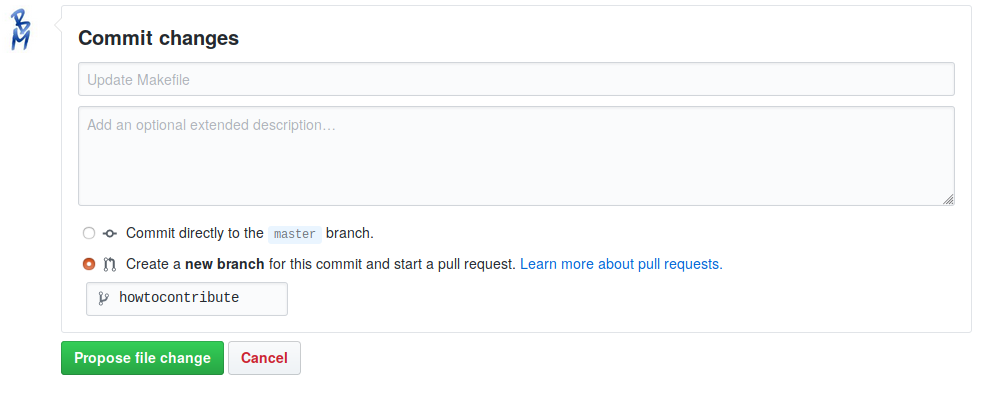
\includegraphics[width=0.8\linewidth]{modif_online_commit.png}
        \end{figure}
        \item Une page de Pull Request s'ouvre, il ne faut pas en tenir compte car elle propose de modifier votre propre répertoire et non le répertoire officiel.
        \item Retourner sur votre répertoire \url{https://github.com/pseudonym/Syntheses}
     \end{wideitemize}
\end{frame}

\begin{frame}
\label{PR}
    \frametitle{Contribuer sans connaître Git - Les Pull Requests}
    \begin{wideitemize}
        \item Dans votre répertoire GitHub, accédez à vos branches
            \begin{figure}[H]
                \centering
                
\includegraphics[width=\linewidth]{modif_online_branches.png}
            \end{figure}
        \item Au niveau de la ligne associée à la branche nouvellement créée, cliquer sur New pull request
            \begin{figure}[H]
                \centering
                
\includegraphics[width=\linewidth]{modif_online_PR.png}
            \end{figure}
         \item Donner une explication sur le contenu de votre Pull Request
         \item Créer la Pull Request
            \begin{figure}[H]
                \centering
                \includegraphics[width=\linewidth]{create_pull_request.png}
            \end{figure}
     \end{wideitemize}
\end{frame}

\section{Contribuer avec \texttt{Git}}

\begin{frame}
    \frametitle{Contribuer avec \texttt{Git}}
    Pour des ajouts de documents ou des grandes modifications, il faut utiliser \texttt{Git}.
    \begin{wideitemize}
         \item Forker le repo officiel (section \ref{fork})
         \item Cloner le fork en local (section \ref{clone_fork})
         \item Pour \textbf{modifier un document existant}, aller directement à la page \ref{modif_local}
         \item Pour \textbf{ajouter un nouveau document}, il faut d'abord générer son template avec le script \texttt{add.sh}
     \end{wideitemize}
\end{frame}

\begin{frame}
    \frametitle{Contribuer avec \texttt{Git}}
    \begin{wideitemize}
         \item Le descriptif des commandes de \texttt{add.sh} est donné à la section \ref{addsh} (ou en tapant \lstinline[mathescape]|bash add.sh| sans argument). 
         
         Par exemple, taper 
         
         \lstinline[mathescape]|bash add.sh 1 info EPL 1401 exam 1997 Juin All| 
         
         pour générer le template de l'examen de juin 1997 en \textit{EPL1401 - Informatique}. 
        
         Le document \LaTeX sera ainsi créé dans \lstinline[mathescape]|src/q1/info-EPL1401/exam/1997/Juin/All|.
     \end{wideitemize}
\end{frame}

\begin{frame}
\label{modif_local}
    \frametitle{Contribuer avec \texttt{Git}}
    \begin{wideitemize}
         \item Faire les modifications désirées dans votre dossier en local.
         \item Ensuite, taper \lstinline[mathescape]|git checkout -b infoepl1104| pour créer une nouvelle branche nommée \lstinline[mathescape]|infoepl1104|.
         \item La commande \lstinline[mathescape]|git status| permet de visualiser tous les documents modifiés/ajoutés.
         \item Taper \lstinline[mathescape]|git add .| et puis
         
         \texttt{git commit -m "Ajout de l'examen d'EPL1401 de Juin 1997"} pour ajouter tous les documents modifiés et nommer le commit.
         \item Taper \lstinline[mathescape]|git push origin infoepl1104| pour mettre la branche sur GitHub.
     \end{wideitemize}
\end{frame}

\begin{frame}
    \frametitle{Contribuer avec \texttt{Git}}
    \begin{wideitemize}
         \item Taper \lstinline[mathescape]|git checkout master| pour revenir sur votre branche master.
         \item Finalement, la proposition de Pull Request se fait sur GitHub, en suivant les indications de la page \ref{PR}.
     \end{wideitemize}
Pour toute question, utiliser 
    \begin{wideitemize}
         \item Les issues: \url{https://github.com/Gp2mv3/Syntheses/issues}
         \item ou le chat Gitter: \url{https://gitter.im/Gp2mv3/Syntheses}
     \end{wideitemize}
    \begin{figure}[H]
        \centering
        
\includegraphics[width=0.3\linewidth]{github-logo.jpg}
    \end{figure}
\end{frame}

\end{document}
